\documentclass[11pt, oneside]{article}   	% use "amsart" instead of "article" for AMSLaTeX format
%\documentclass{splib}
\usepackage{geometry}                		% See geometry.pdf to learn the layout options. There are lots.
\geometry{letterpaper}                   		% ... or a4paper or a5paper or ... 
%\geometry{landscape}                		% Activate for for rotated page geometry
%\usepackage[parfill]{parskip}    		% Activate to begin paragraphs with an empty line rather than an indent
\usepackage{graphicx}				% Use pdf, png, jpg, or eps with pdflatex; use eps in DVI mode
								% TeX will automatically convert eps --> pdf in pdflatex		
\usepackage{amssymb,amsmath}
\usepackage{sidecap}
\usepackage{wrapfig}
\usepackage{float}
\usepackage{caption}
\usepackage{subcaption}
\usepackage{url}
\usepackage{verbatim} 
\usepackage[toc,page]{appendix}
\usepackage{ifthen}
\usepackage{listings}
\numberwithin{equation}{section}
\title{Privacy Limit Theorem}
\author{Sashank Dara } 

\begin{document}

\maketitle
\abstract{
With the explosion in the data being collected some believe privacy is dead. With advances in privacy technologies like homomorphic encryption, differential privacy etc. some believe we are closer to the holy grail of privacy applications. \emph{Privacy} and \emph{Utility} are not necessarily to two orthogonal entities.  Few argue  both cannot exist  together and few believe otherwise. The truth is some where in between.  This talks tries to debunk many myths surrounding  \emph{privacy preserving technologies} like computation over encrypted data, differential privacy etc. Using real world examples, the talk explores the fundamental limitations on how much privacy can be achieved. Maximum utility of the data leads to zero privacy and total privacy erodes the utility of the data completely. The spectrum of opportunity lies in between which modern privacy preserving technologies try to leverage. It is also important to understand the theoretical limitations.  This talk explores the fundamental limits of privacy that could be achieved without eroding the utility of the data and conjectures a {\bf \emph{Privacy Limit Theorem}}.
}
\section{Privacy }

Data is essential for any meaningful insights at the same time privacy is important.  Can we have the data and privacy both together ? Yes and No. Lets take a step back to understand what is privacy ? 

There are two fundamental aspects to it that are often confused to be same.
\begin{enumerate}
\item \emph {Data Privacy:} Hiding the data from the entity that is processing it ?
\item \emph{Identity Privacy:} Hiding the \emph{identity}\footnote{Identity could be names, emotions, religious preferences, political opinions etc.} of an individual in the given data ?
\end{enumerate}

\subsection{Data Privacy}

Can we encrypt the data and still compute on it without decrypting it ? Computations could be specialised operations like search, sort or advanced operations like machine learning, analytics. Many researchers are building efficient solutions for this problem domain collectively being called as COED (Computation over encrypted Data). It is heavily being sensationalised that its impact on Cloud, IOT and other technologies would be humongous. Every advance in areas like \emph{ homomorphic encryption, secure multiparty computation, searchable encryption etc} are hailed as a step closer to holy grail. At this moment it is very important to understand the limits of data privacy, collectively this technology could offer (irrespective of the advances on efficiency). 

The strongest \emph{data privacy} any traditional encryption scheme could achieve is \emph{adaptive ciphertext indistinguishability (IND-CCA2)}  also called as \emph{semantic security}. Informally this means an attacker cannot distinguish pairs of \emph{ciphertext} based on the message they encrypt even if they could interact with encryption/decryption oracles. This is not true for encryption schemes that enable computation over encrypted data. For example, the strongest privacy a \emph{fully homomorphic encryption} scheme can achieve is \emph{non-adaptive ciphertext indistinguishability (IND-CCA1)}. Informally this means an attacker can distinguish pairs of \emph{ciphertext} based on the message they encrypt if they are allowed to interact with encryption/decryption oracles. 

So technically encryption schemes that preserve the utility even after encryption offer lesser privacy than schemes that do not preserve any utility. (More realistic examples to be followed in the talk)


\subsection{Identity Privacy}
Can we hide the identity of the person in a corpus of data ? A promising approach is \emph{differential privacy}. 
This technology offers a \emph{privacy budget} to hide identity of individuals in \emph{statistical databases} by adding\emph{carefully} defined statistical noise. This helps in querying these databases without providing the ability to link the identity of the person with the query results (thus providing \emph{identity privacy}) within a reasonable privacy budget $\epsilon$.

It is very important to understand the \emph{utility-privacy} trade off here. The maximum \emph{utility} that could be derived from these databases is achieved when no such noise is added. On the other hand random addition of noise would considerably deteriorate the quality of the query results (one could argue that it might offer better privacy since the database is meaningless). Now \emph{differential privacy} offers a well calculated noise levels that retains the utility. The nuance is that not all queries could be performed after adding $\epsilon$ (thus constraining the utility). 

Lets take an example, a mobile application developer may want to understand the frequency  of \emph{emoji}s to improve user experience (like placing them appropriately etc.). The usage could be collected by the app and sent to a remote server for analysis across many users. The precise privacy breach is such data would reveal the individual's emotional state (happy/sad etc.) based on their frequently used \emph{emoji's}.  In order to protect the individual's privacy, \emph{differential privacy} could be used and certain amount of calculated noise could be added to the frequency of the usage. 

At very high level, if the noise added is too high the privacy of individual could be protected well but the frequency of usage gets distorted and cannot be used. If the noise added is too low the mobile application provider could breach the privacy of the user. Irrespective of the level of noise, it is very easy to determine the emotional state if at all the data is of any real use.  

\section{Privacy Limit Theorem}

\emph{Privacy} and \emph{Utility} are considered to be two orthogonal entities. Either we could achieve complete privacy of the data by encrypting  or we have complete utility of the data. The talk conjectures the modern privacy preserving technologies have a only a small  window of opportunity to achieve real world privacy.

\begin{figure}
  \begin{center}
    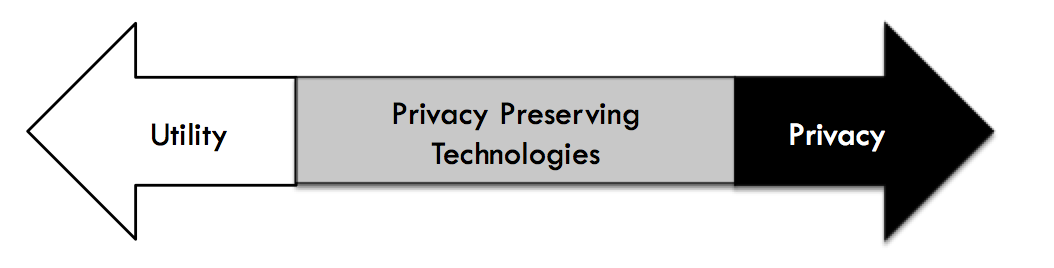
\includegraphics[width=0.7\textwidth]{conflict.png}
  \caption{Conflict and Window of Opportunity }
    \end{center}
\end{figure}

\section{Conclusions}
The privacy utility trade off is conjectured as \emph{privacy limit theorem}. Informally it states that the utility erodes while increasing levels of privacy is achieved and privacy erodes when the utility that could be derived from data increases. The spectrum of opportunity for privacy preserving technologies is some where in between. 
 
\end{document}  